\section*{Exercise (vi)}

We simulate $N = 1000$ paths of the life annuity benefit $Y(t)$ for $t \in [m, 111]$ using an Euler scheme with step length $h = 1/100$ on the dynamics derived in Exercise~(v):
\[
  \mathrm{d}Y(t) = \bigl(\pi(t)\alpha + (1-\pi(t))r - \tilde{r}(t) + \mu(t) - \tilde{\mu}(t)\bigr)\,Y(t)\,\mathrm{d}t + \sigma\pi(t)\,Y(t)\,\mathrm{d}W(t).
\]
With the calculation basis from Table~2 the drift coefficient vanishes, so the Euler step reduces to
\[
  Y(t_{i+1}) = Y(t_i) + \sigma\,\pi(t_i)\,Y(t_i)\,\sqrt{h}\,Z_i, \qquad Z_i \overset{\mathrm{iid}}{\sim} N(0,1).
\]
The initial value is $Y(m) = X(m)/\tilde{V}_0(m)$, where $X(m) \approx 9{,}821{,}181$ is taken from the simulated path in Exercise~(ii), giving $Y(70) \approx 827{,}421$. The dashed line in the figure marks this initial benefit level. A selection of 15 sample paths is shown below.

\begin{figure}[H]
    \centering
    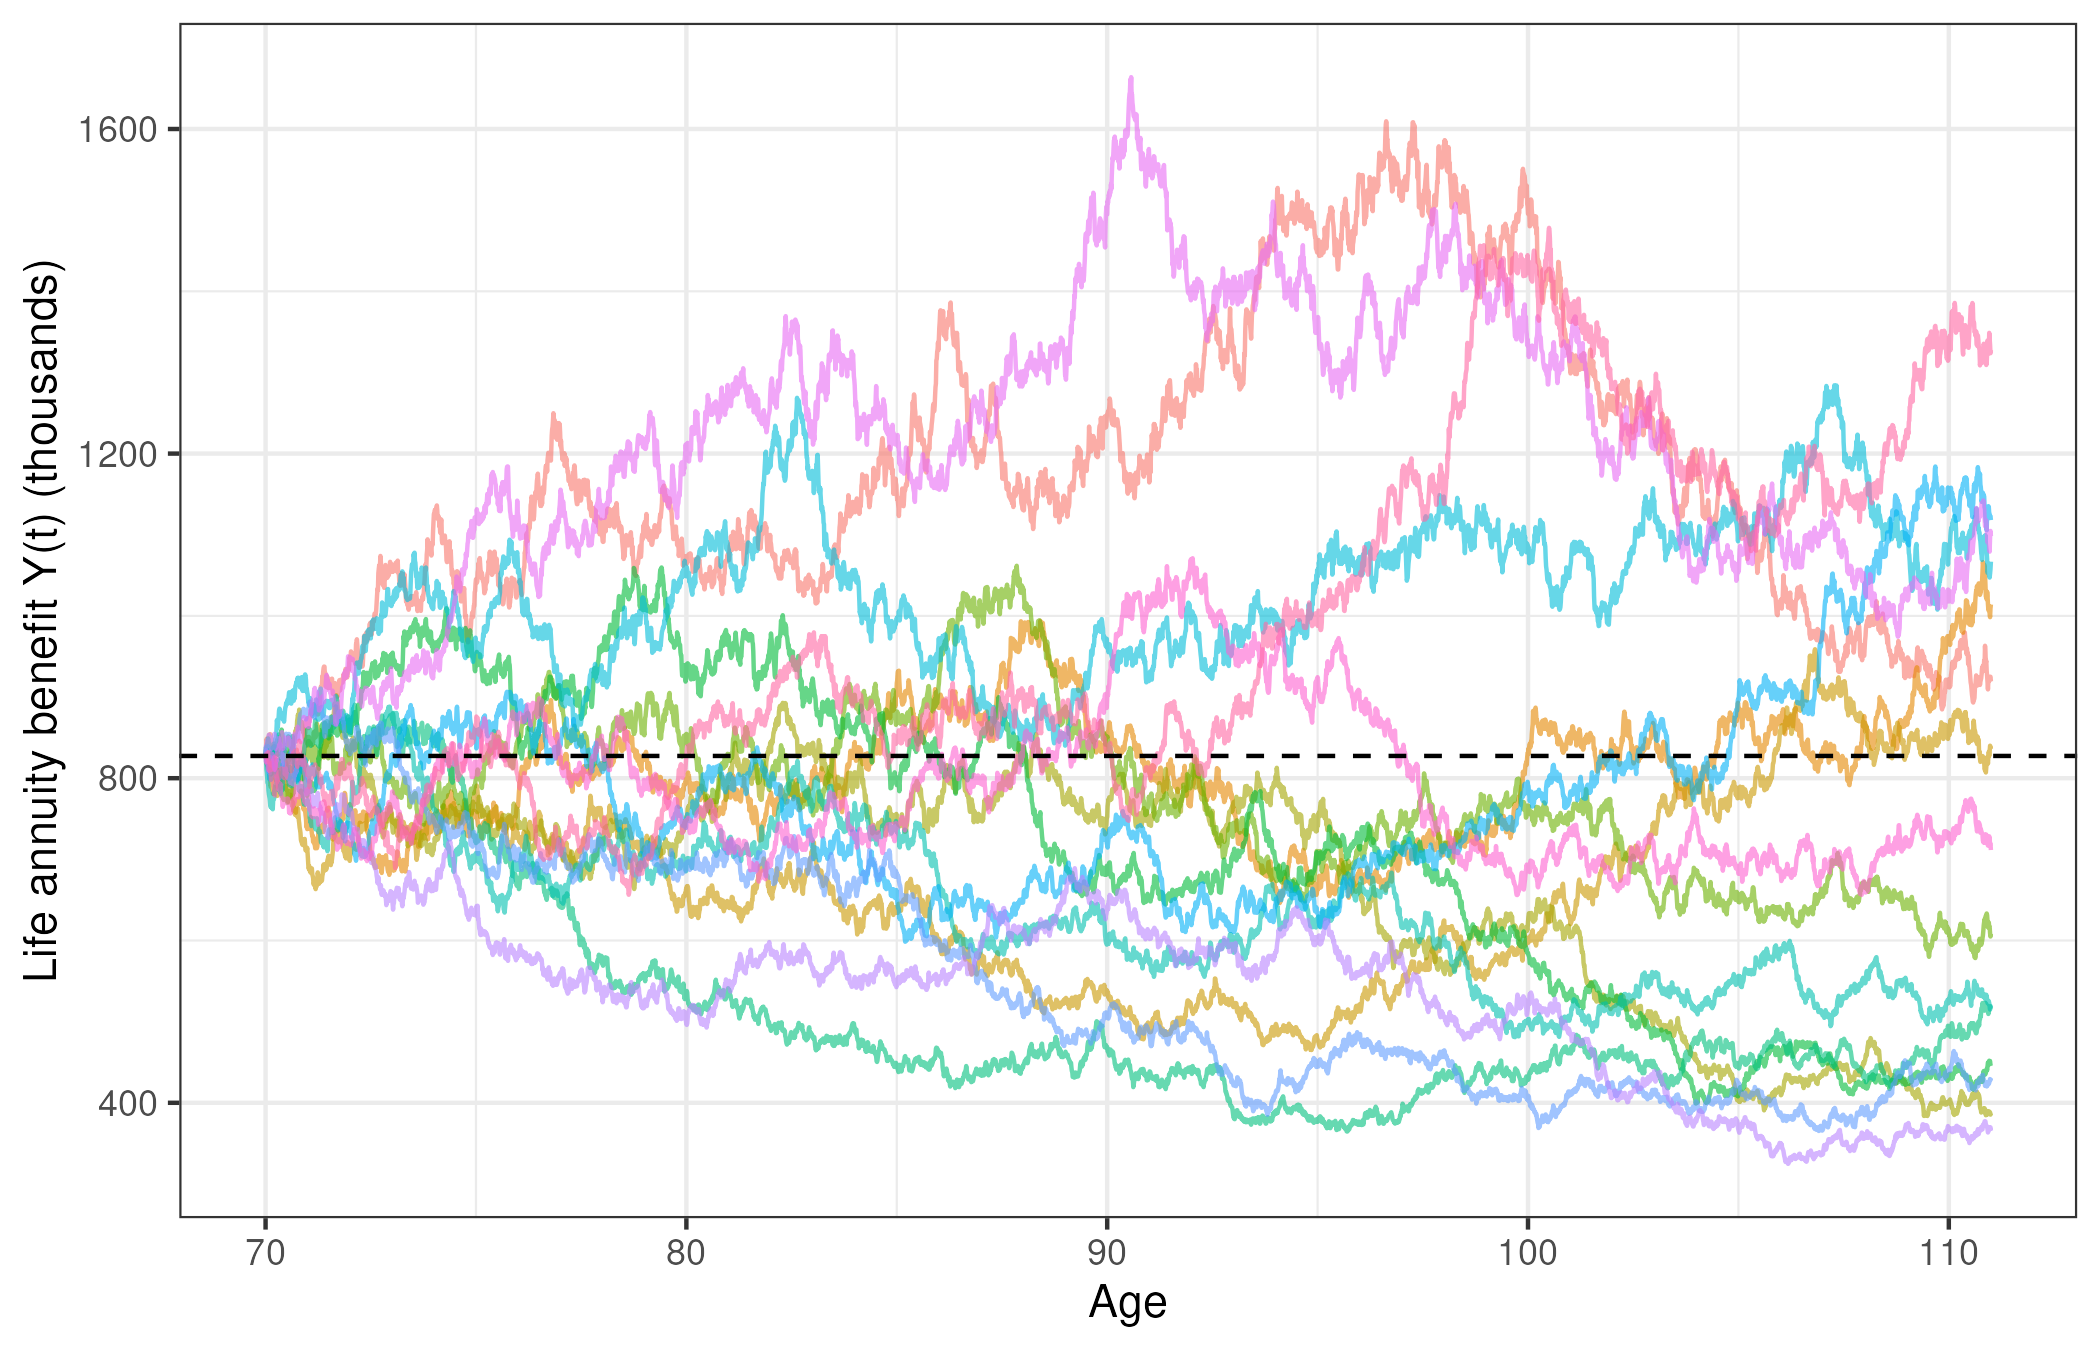
\includegraphics[width=0.75\linewidth]{Pictures/AnnuitySamplePaths.png}
    \caption{15 simulated paths of the life annuity benefit $Y(t)$. The dashed line marks the initial benefit $Y(m)$.}
\end{figure}

We observe significant variation across paths: some paths see benefits double or more, while others decline substantially. This dispersion reflects the stochastic investment risk borne by the insured under the unit-link design.

